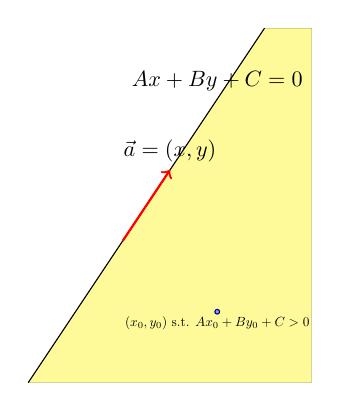
\begin{tikzpicture}[scale=.6, every node/.style={scale=.8}]
	\coordinate (hp0) at (-2,-4);
	\coordinate (hp1) at (3,3.5);
	\filldraw[ultra thin,draw=yellow!50!black,fill=yellow!40!white] (hp0) -- (hp1) -- (4,3.5) -- (4,-4) -- (hp0);
	\draw[thin] (hp0) -- (hp1);

	\drawcsys{-3.5}{4}{-4}{3.5}

	\coordinate (v0) at (0,-1);
	\coordinate (v1) at (1,.5);
	\draw[thick,->,draw=red] (v0) -- (v1) node[above]{\(\vec{a}=(x,y)\)};

	\coordinate (p0) at (2,-2.5);
	\filldraw[thin,draw=blue!50!black,fill=blue!40!white] (p0) circle[radius=.05];
	\draw (p0) node[scale=.6,below]{\((x_0,y_0)\) s.t. \(Ax_0+By_0+C>0\)};

	\coordinate (p1) at (2,2);
	\draw (p1) node[above]{\(Ax+By+C=0\)};
\end{tikzpicture}
